\documentclass[11pt,a4paper]{article}
\usepackage[spanish,es-nodecimaldot]{babel}	% Utilizar español
\usepackage[utf8]{inputenc}					% Caracteres UTF-8
\usepackage{graphicx}						% Imagenes
\usepackage[hidelinks]{hyperref}			% Poner enlaces sin marcarlos en rojo
\usepackage{fancyhdr}						% Modificar encabezados y pies de pagina
\usepackage{float}							% Insertar figuras
\usepackage[textwidth=390pt]{geometry}		% Anchura de la pagina
\usepackage[nottoc]{tocbibind}				% Referencias (no incluir num pagina indice en Indice)
\usepackage{enumitem}						% Permitir enumerate con distintos simbolos
\usepackage[T1]{fontenc}					% Usar textsc en sections
\usepackage{amsmath}						% Símbolos matemáticos
\usepackage{listings}
\usepackage{color}

 
\definecolor{codegreen}{rgb}{0,0.6,0}
\definecolor{codegray}{rgb}{0.5,0.5,0.5}
\definecolor{codepurple}{rgb}{0.58,0,0.82}
\definecolor{backcolour}{rgb}{0.99,0.99,0.99}
 
\lstdefinestyle{mystyle}{
    backgroundcolor=\color{backcolour},   
    commentstyle=\color{codegreen},
    keywordstyle=\color{magenta},
    numberstyle=\tiny\color{codegray},
    stringstyle=\color{codepurple},
    basicstyle=\footnotesize,
    breakatwhitespace=false,         
    breaklines=true,                 
    captionpos=b,                    
    keepspaces=true,                 
    numbers=left,                    
    numbersep=5pt,                  
    showspaces=false,                
    showstringspaces=false,
    showtabs=false,                  
    tabsize=2
}
 
\lstset{style=mystyle, language=Python}

% Comando para poner el nombre de la asignatura
\newcommand{\asignatura}{Inteligencia de Negocio}
\newcommand{\autor}{José María Sánchez Guerrero}
\newcommand{\titulo}{Práctica 1}
\newcommand{\subtitulo}{Resolución de problemas de clasificación y análisis experimental.}

% Configuracion de encabezados y pies de pagina
\pagestyle{fancy}
\lhead{\autor{}}
\rhead{\asignatura{}}
\lfoot{Grado en Ingeniería Informática}
\cfoot{}
\rfoot{\thepage}
\renewcommand{\headrulewidth}{0.4pt}		% Linea cabeza de pagina
\renewcommand{\footrulewidth}{0.4pt}		% Linea pie de pagina

\begin{document}
\pagenumbering{gobble}

% Pagina de titulo
\begin{titlepage}

\begin{minipage}{\textwidth}

\centering

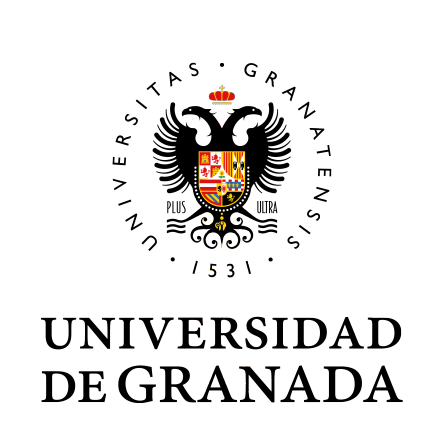
\includegraphics[scale=0.5]{img/ugr.png}\\

\textsc{\Large \asignatura{}\\[0.2cm]}
\textsc{GRADO EN INGENIERÍA INFORMÁTICA}\\[1cm]

\noindent\rule[-1ex]{\textwidth}{1pt}\\[1.5ex]
\textsc{{\Huge \titulo\\[0.5ex]}}
\textsc{{\Large \subtitulo\\}}
\noindent\rule[-1ex]{\textwidth}{2pt}\\[3.5ex]

\end{minipage}

\vspace{0.5cm}

\begin{minipage}{\textwidth}

\centering

\textbf{Autor}\\ {\autor{}}\\[2.5ex]
\textbf{Rama}\\ {Sistemas de Información}\\[2.5ex]
\vspace{0.3cm}


\includegraphics[scale=0.3]{img/etsiit.jpeg}

\vspace{0.3cm}
\textsc{Escuela Técnica Superior de Ingenierías Informática y de Telecomunicación}\\
\vspace{1cm}
\textsc{Curso 2020-2021}
\end{minipage}
\end{titlepage}

\pagenumbering{arabic}
\tableofcontents
\thispagestyle{empty}				% No usar estilo en la pagina de indice

\newpage

\setlength{\parskip}{1em}



\section{Introducción}

En este trabajo vamos a analizar el comportamiento de distintos algoritmos de clasificación en el problema propuesto. Disponemos
de un dataset, llamado \textit{''Mammographic Mass dataset''}, en el cual se desea predecir el tipo de tumor (benigno o maligno)
en una serie de mamografías realizadas para un estudio sobre el cáncer de mama. Este estudio lo vamos a realizar gracias a los
siguientes atributos proporcionados en el dataset:

\begin{itemize}
	\item \textbf{BI-RADS.} Este parámetro representa un control de calidad de las mamografías. Consta de 7 categorías distintas,
		  en las que, cuanto más alto sea el valor, hay una mayor probabilidad de que sea maligno.

	\item \textbf{Edad} del paciente.
	
	\item \textbf{Forma de la masa.} Dependiendo de como sea la masa anormal detectada, se clasifica como \textbf{R}edondeada,
		  \textbf{O}valada, \textbf{L}obulada, \textbf{I}rregular ó \textbf{N}o definida.

	\item \textbf{Margen de masa.} Circumscribed = 1, microlobulated = 2, obscured = 3, ill-defined = 4, spiculated = 5 (nominal).
	
	\item \textbf{Densidad de la masa.} Valores entre 1 y 4, siendo 1 la más alta y 4 contenido graso (no tumoral).
	
	\item \textbf{Severidad.} Es el atributo que se desea predecir, es decir, si es un tumor benigno o maligno.	

\end{itemize}

En el dataset hay datos de 961 pacientes, sin embargo, nos gustaría dejar un porcentaje para validar el modelo y así ver cómo va
entrenando los datos. Posteriormente, se explicará cómo se ha determinado qué datos son los de entrenamiento y cuáles son los de
test.

\newpage

\section{Procesado de datos}

Lo primero que tenemos que hacer es mostrar varios de los datos que tenemos y analizarlos. En mi caso vamos a sacar las 5 primeras
filas:

\begin{table}[H]
    \centering
    \resizebox{\textwidth}{!}{%
    \begin{tabular}{|c|c|c|c|c|c|c|}
    \hline
    \textbf{} & \textbf{BI-RADS} & \textbf{Age} & \textbf{Shape} & \textbf{Margin} & \textbf{Density} & \textbf{Severity} \\ \hline
    \textbf{0} & 5.0 & 67.0 & L & 5.0 & 3.0 & maligno \\ \hline
    \textbf{1} & 4.0 & 43.0 & R & 1.0 & NaN & maligno \\ \hline
    \textbf{2} & 5.0 & 58.0 & I & 5.0 & 3.0 & maligno \\ \hline
    \textbf{3} & 4.0 & 28.0 & R & 1.0 & 3.0 & benigno \\ \hline
    \textbf{4} & 5.0 & 74.0 & R & 5.0 & NaN & maligno \\ \hline
    \end{tabular}%
    }
\end{table}

Podemos observar que tenemos tanto datos numéricos, como datos categóricos, como ya comentamos en la introducción. También podemos
observar que tenemos varias celdas con datos erróneos o perdidos (representados con el valor $NaN$), por lo que será importante
procesarlos para que nuestros algoritmos funcionen correctamente. Primero veamos qué cantidad de estos datos nulos tenemos:

\begin{table}[H]
    \centering
    \begin{tabular}{|l|l|}
    \hline
    \multicolumn{1}{|c|}{\textbf{BI-RADS}} & 2 \\ \hline
    \textbf{Age} & 5 \\ \hline
    \textbf{Shape} & 0 \\ \hline
    \textbf{Margin} & 48 \\ \hline
    \textbf{Density} & 76 \\ \hline
    \textbf{Severity} & 0 \\ \hline
    \end{tabular}
\end{table}

Son una cantidad bastante alta de datos, en comparación con la cantidad de datos totales que tenemos. Por lo tanto, eliminar toda
las filas que contengan uno, puede dejarnos con muy pocos datos para entrenar y validar, y que el modelo sea más débil. No obstante,
el introducir datos para reemplazar uno faltante ha de realizarse con cuidado, ya que no son datos reales.

También tenemos que tener en cuenta cuál es la distribución de estos datos antes de trabajar con ellos. Es decir, tenemos que
asegurarnos de no sesgar nuestros datos si los eliminamos. Si hay algún tipo de correlación, tendríamos que intentar completarlos
de alguna forma. Para ello, vamos a generar una gráfica para cada uno de los atributos del $dataset$, en la que mostraremos la
cantidad de datos antes y después de eliminarlos, y asi ver cómo están distribuidos.

\newpage
Los resultados son los siguientes:

\begin{figure}[H]
\centering

\begin{minipage}{0.5\textwidth}
    \centering
    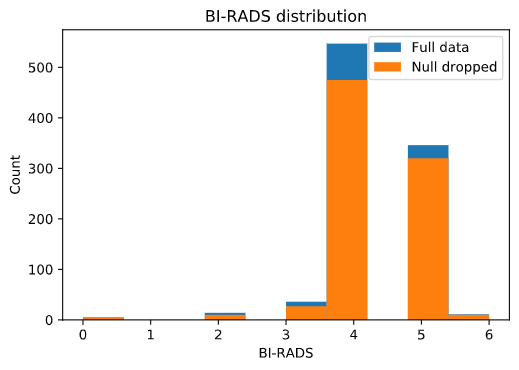
\includegraphics[scale=0.35]{img/birads-distribution.png}
\end{minipage}%
\begin{minipage}{0.5\textwidth}
    \centering
    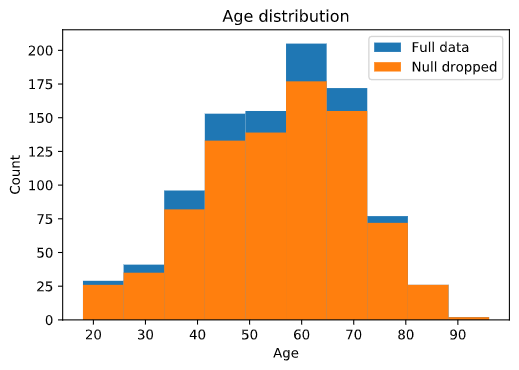
\includegraphics[scale=0.35]{img/age-distribution.png}
\end{minipage}

\end{figure}


\begin{figure}[H]
\centering

\begin{minipage}{0.5\textwidth}
    \centering
    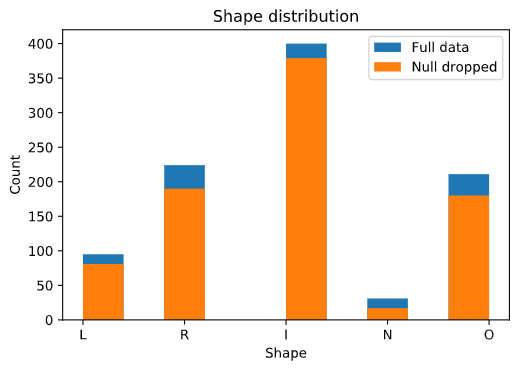
\includegraphics[scale=0.35]{img/shape-distribution.png}
\end{minipage}%
\begin{minipage}{0.5\textwidth}
    \centering
    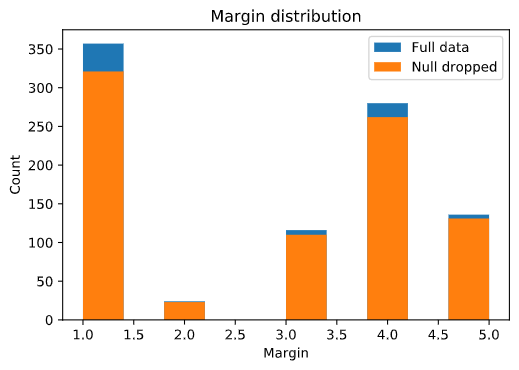
\includegraphics[scale=0.35]{img/margin-distribution.png}
\end{minipage}

\end{figure}


\begin{figure}[H]
\centering

\begin{minipage}{0.5\textwidth}
    \centering
    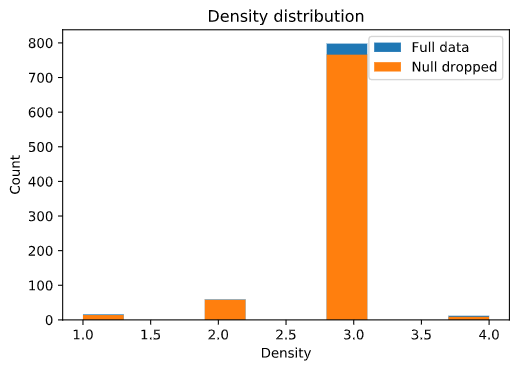
\includegraphics[scale=0.35]{img/density-distribution.png}
\end{minipage}%
\begin{minipage}{0.5\textwidth}
    \centering
    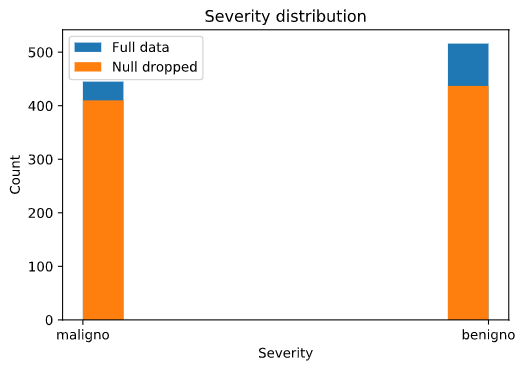
\includegraphics[scale=0.35]{img/severity-distribution.png}
\end{minipage}

\end{figure}

Podemos observar que los datos nulos están distribuidos aleatoriamente entre los atributos, por lo que podremos eliminarlos del
$dataset$ sin ningún problema (y teniendo en cuenta que tendremos menos datos para trabajar).

% PROBAR REEMPLAZANDO LOS DATOS CON ALEATORIOS
% \textit{Pandas} nos proporciona la función ''\textit{fillna()}'' para reemplazar los valores faltantes con un valor específico



\section{Configuración de algoritmos}
Para todos los algoritmos hemos procedido de la misma manera, y así evaluarlos a todos en igualdad de condiciones. Para comenzar,
declaramos el clasificador con sus parámetros correspondientes (en nuestro caso, las primeras evaluaciones han sido con los
parámetros por defecto y una semilla $random\_state=0$).

Posteriormente, hacemos las predicciones correspondientes para los datos de entrenamiento. Lo hacemos mediante validación cruzada
de 5 particiones, gracias a la función:
$$cross\_val\_predict(classifier, x\_train, y\_train, cv=5)$$

Por último, para evaluar los resultados obtenidos vamos a usar:
\begin{itemize}
    \item \textbf{Classification report.} Crea un informe que muestra las principales métricas de clasificación: precisión, recall,
          f1-score, y promedios macro, ponderado y de la muestra.
    \item \textbf{Score.} Misma medida del informe anterior mostrada con un poco más de precisión.
    \item \textbf{Confusion matrix.} Muestra una matriz para evaluar la precisión de la clasificación. Cada fila representa las
          instancias de una clase predicha, mientras que cada columna representa las instancias reales de ésta.
\end{itemize}

Los algoritmos que evaluaremos han sido elegidos porque, cada uno de ellos, tiene una forma de procesar los datos diferente a todos
los demás. Estos algoritmos son los siguientes:


\subsection{K-Nearest-Neighbors (k-NN)}
Comenzamos por este algoritmo ya que es uno de los más utilizados, debido a su simplicidad. Este algoritmo funciona de la siguiente
manera. Cuando tenemos un nuevo ejemplo a clasificar, calcula la distancia (Euclídea) con respecto a los datos ya existentes, y
considerando los $k$ más cercanos, determina si pertenece a una clase u otra.

\newpage
A la hora de implementarlo lo hacemos de la siguiente forma:
$$KnnClf = KNeighborsClassifier(n\_neighbors=5)$$

Seleccionamos un número \textbf{k=5} de vecinos a evaluar y dejamos el resto de parámetros que trae el algoritmo por defecto. El
parámetro anterior es el más relevante, sin embargo, algunos otros interesantes a estudiar pueden ser, por ejemplo: \textbf{p},
que sirve para cambiar el tipo de distancia utilizada (Euclídea, Manhattan o Minkowski); ó \textbf{weights}, que determina la
influencia de los vecinos en la predicción (todos ponderan igual, los cercanos influyen más o tu propia función).

\subsection*{Resultados obtenidos}
% Please add the following required packages to your document preamble:
% \usepackage{graphicx}
\begin{table}[H]
    \centering
    \begin{tabular}{c|cccc}
        \textbf{} & \textbf{precision} & \textbf{recall} & \textbf{f1-score} & \textbf{support} \\ \hline
        \textbf{0} & 0.80 & 0.82 & 0.81 & 347 \\
        \textbf{1} & 0.81 & 0.78 & 0.79 & 330 \\ \hline
        \textbf{accuracy} &  &  & 0.80 & 677 \\
        \textbf{macro avg} & 0.80 & 0.80 & 0.80 & 677 \\
        \textbf{weighted avg} & 0.80 & 0.80 & 0.80 & 677
    \end{tabular}
\end{table}

\begin{figure}[H]
    \centering
    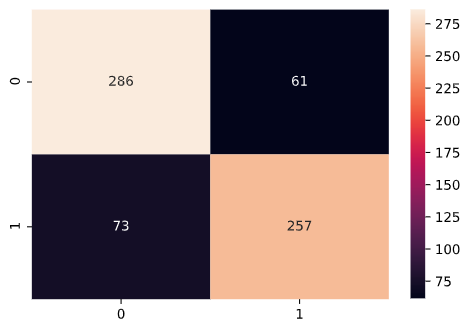
\includegraphics[scale=0.5]{img/matrix-knn.png}    
\end{figure}
\vspace{-20px}
$$\textbf{SCORE:  } 0.7991137370753324$$

\subsection{Decision Tree}
Este clasificador, como su propio nombre indica, es un árbol en el que cada \textbf{hoja} es una clase y cada \textbf{nodo} es
un nodo de decisión con una prueba simple a realizar.

El algoritmo funciona de la siguiente forma. Todos los ejemplos de entrenamiento comienzan desde el nodo raíz y se dividen
recursivamente los ejemplos en base a los atributos seleccionados. Esta selección de atributos se suele realizar mediante el
criterio ''\textit{gini}'', pero también hay otros como ''\textit{InfoGain}'' o ''\textit{GainRatio}''. Posteriormente,
quitamos las ramas con ruido o con datos anómalos.

A la hora de implementarlo lo hacemos de la siguiente forma:
$$DecTreeClf = tree.DecisionTreeClassifier(random_state=0)$$

El parámetro \textbf{random\_state} nos sirve para seleccionar la semilla. El resto de parámetros los dejamos por defecto, ya
que la mayoría son utilizados para limitar el número de hojas, el número de características, etc. que en nuestro ejemplo no
necesitaremos. También tenemos el parámetro \textbf{criterion}, que nos sirve para elegir el criterio de selección de atributos
comentado anteriormente.

\subsection*{Resultados obtenidos}
% Please add the following required packages to your document preamble:
% \usepackage{graphicx}
\begin{table}[H]
    \centering
    \begin{tabular}{c|cccc}
        \textbf{} & \textbf{precision} & \textbf{recall} & \textbf{f1-score} & \textbf{support} \\ \hline
        \textbf{0} & 0.75 & 0.82 & 0.78 & 347 \\
        \textbf{1} & 0.79 & 0.72 & 0.75 & 330 \\ \hline
        \textbf{accuracy} & & & 0.77 & 677  \\
        \textbf{macro avg} & 0.77 & 0.77 & 0.77 & 677 \\
        \textbf{weighted avg} & 0.77 & 0.77 & 0.77 & 677
    \end{tabular}
\end{table}

\begin{figure}[H]
    \centering
    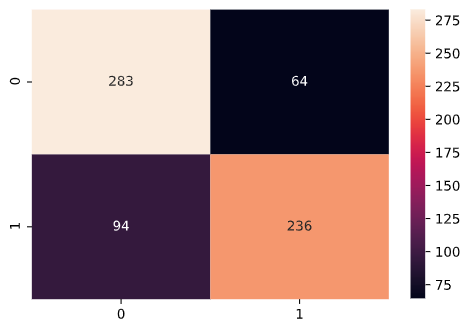
\includegraphics[scale=0.5]{img/matrix-tree.png}    
\end{figure}
$$\textbf{SCORE:  } 0.7666174298375185$$


\subsection{Naive-Bayes}
Se ha utilizado porque es el modelo de red bayesiana orientada a clasificación más simple. Este algoritmo se considera un
estándar y sus resultados son competitivos, pese a utilizar una hipótesis poco realista. Es decir, suponemos que todos los
atributos son independientes a partir de su clase, asi que la hipótesis MAP (Máximo a posteriori) en un Naive-Bayes queda así:
$$C_{MAP} = \arg _{c\epsilon \Omega_C}maxP(c|a_1,...,a_n) = \arg _{c\epsilon \Omega_C}maxP(c)\prod_{i=1}^{n}P(a_i|c)$$

En la práctica, existen dependencias entre variables, por lo que puede llevar a una falta de precisión que no se puede retocar
en un clasificador como este (existen redes de creencia bayesianas para solucionar esto).

A la hora de implementarlo lo hacemos de la siguiente forma:
$$GaussianClf = GaussianNB()$$

No ponemos ningún parámetro ya que es un clasificador que no se puede modelar o retocar, como acabamos de decir.

\subsection*{Resultados obtenidos}
% Please add the following required packages to your document preamble:
% \usepackage{graphicx}
\begin{table}[H]
    \centering
    \begin{tabular}{c|cccc}
        \textbf{} & \textbf{precision} & \textbf{recall} & \textbf{f1-score} & \textbf{support} \\ \hline
        \textbf{0} & 0.85 & 0.78 & 0.81 & 347 \\
        \textbf{1} & 0.79 & 0.85 & 0.82 & 330 \\ \hline
        \textbf{accuracy} & & & 0.82 & 677 \\
        \textbf{macro avg} & 0.82 & 0.82 & 0.82 & 677 \\
        \textbf{weighted avg} & 0.82 & 0.82 & 0.82 & 677
    \end{tabular}
\end{table}

\begin{figure}[H]
    \centering
    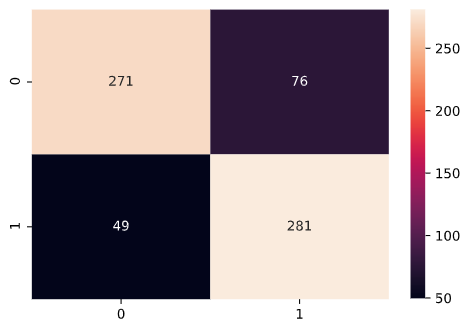
\includegraphics[scale=0.5]{img/matrix-naivebayes.png}    
\end{figure}
$$\textbf{SCORE:  } 0.8153618906942393$$


\subsection{Neural Network}
Estos algoritmos están basados en los propios sistemas nerviosos biológicos:
\begin{figure}[H]
    \centering
    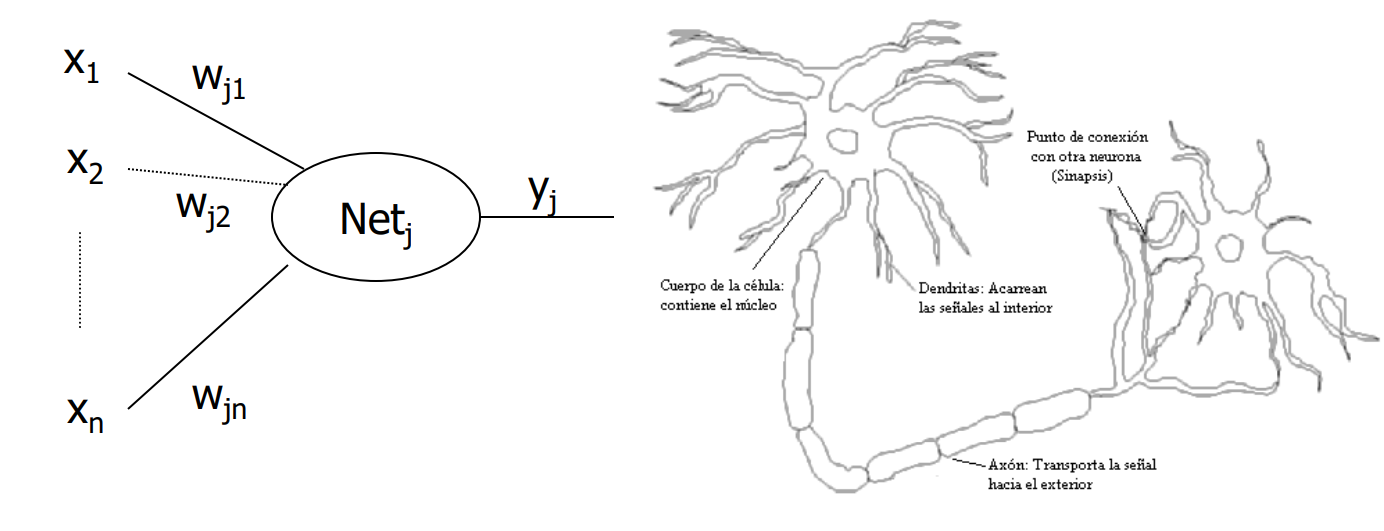
\includegraphics[scale=0.38]{img/neural-network.png}    
\end{figure}

Como podemos ver en la figura, cada señal que llega a las dendritas \{$x_1,x_2,...,x_n$\} serían nuestros datos de entrada
del modelo. Las sinapsis o puntos de conexión con otra neurona, serían los pesos \{$w_1,w_2,...,w_n$\} que ponderan a las
entradas: \textbf{positivo} es una sinapsis excitadora y \textbf{negativo} es una sinapsis inhibidora.

Después, la actividad interna de cada célula sería la sumatoria entre cada una de las conexiones anteriores, y por último, la
\textbf{función de activación} que, dadas estas entradas, define una salida para el modelo:
$$y_j = f(Net_j - \theta_j) = f(\sum w_{ji} \cdot x_i - \theta)$$

Para este trabajo, no vamos a implementar una red neuronal desde cero, ya que es una tarea bastante compleja. Sin embargo,
vamos a utilizar un \textbf{MultiLayer Perceptron (MLP)}, que es una red neuronal compuesta por: una capa de entrada, capas
ocultas (o \textit{hidden layers}) y una capa de salida. Excepto los datos de entrada, cada nodo es una neurona que utiliza
una función de activación no lineal (sigmoidal es la más común), y en el entrenamiento utiliza la técnica de \textit{backtracking}

A la hora de implementarlo lo haremos de la siguiente forma:
$$PerceptronClf = MLPClassifier(hidden\_layer\_sizes=100, random\_state=0)$$

Aquí podemos ver la cantidad de capas ocultas que queremos que tenga nuestra red. Es el parámetro más importante, ya que
cuanto más alto sea, más aprenderá de los datos que tenemos. Esto no quiere decir que tengamos que poner un valor muy alto,
ya que puede causar sobreaprendizaje en nuestro modelo. El otro parámetro que aparece, al igual que en los otros clasificadores,
nos sirve para seleccionar la semilla.

También existen otros parámetros importantes, como pueden ser: \textbf{activation}, con la que podemos seleccionar la función
de activación a utilizar; \textbf{early\_stopping}, que sirve para finalizar el entrenamiento si no se mejora durante un número
X de iteraciones; o parámetros relacionados con los pesos como \textbf{solver} (para la optimización de los pesos), \textbf{
learning\_rate} (tasa de aprendizaje) ó \textbf{tol} (tolerancia).

\subsection*{Resultados obtenidos}
% Please add the following required packages to your document preamble:
% \usepackage{graphicx}
\begin{table}[H]
    \centering
    \begin{tabular}{c|cccc}
        \textbf{} & \textbf{precision} & \textbf{recall} & \textbf{f1-score} & \textbf{support} \\ \hline
        \textbf{0} & 0.82 & 0.87 & 0.85 & 347 \\
        \textbf{1} & 0.86 & 0.80 & 0.83 & 330 \\ \hline
        \textbf{accuracy} & & & 0.84 & 677 \\
        \textbf{macro avg} & 0.84 & 0.84 & 0.84 & 677 \\
        \textbf{weighted avg} & 0.84 & 0.84 & 0.84 & 677
    \end{tabular}
\end{table}

\begin{figure}[H]
    \centering
    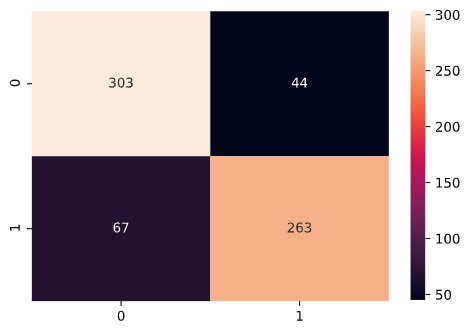
\includegraphics[scale=0.5]{img/matrix-neuralnetwork.png}    
\end{figure}
$$\textbf{SCORE:  } 0.8360413589364845$$

\subsection{Support Vector Machine (SVM)}
El último algoritmo que vamos a utilizar es uno de los más populares en cuanto a la clasificación binaria. Una SVM construye
un hiperplano entre las dos clases de forma que la separación entre ellas se amplie al máximo. Se van transformando los datos
de entrada en un espacio de caracteristicas mediante el \textbf{producto interno (escalar)}.

A la hora de implementarlo lo haremos de la siguiente forma:
$$SvmClf = SVC(random\_state=0, gamma='auto')$$

El primer parámetro que tenemos aquí es la semilla, al igual que en los otros. El siguiente parámetro es para seleccionar
el coeficiente del \textbf{kernel} (el cual también es otro parámetro que también se podrá modificar).

También tenemos otros parámetros como son la \textbf{C}, para la regularazación; \textbf{tol} o tolerancia, como en las redes
neuronales; o hasta un \textbf{max\_iter} por si queremos poner un máximo de iteraciones.

\subsection*{Resultados obtenidos}
% Please add the following required packages to your document preamble:
% \usepackage{graphicx}
\begin{table}[H]
    \centering
    \begin{tabular}{c|cccc}
        \textbf{} & \textbf{precision} & \textbf{recall} & \textbf{f1-score} & \textbf{support} \\ \hline
        \textbf{0} & 0.81 & 0.88 & 0.84 & 347 \\
        \textbf{1} & 0.86 & 0.78 & 0.82 & 330 \\ \hline
        \textbf{accuracy} & & & 0.83 & 677 \\
        \textbf{macro avg} & 0.83 & 0.83 & 0.83 & 677 \\
        \textbf{weighted avg} & 0.83 & 0.83 & 0.83 & 677
    \end{tabular}
\end{table}

\begin{figure}[H]
    \centering
    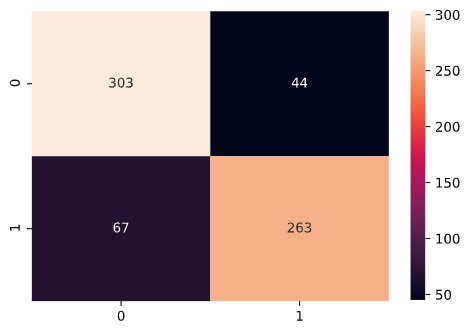
\includegraphics[scale=0.5]{img/matrix-neuralnetwork.png}    
\end{figure}
$$\textbf{SCORE:  } 0.8301329394387001$$



\newpage
\section{Análisis de los resultados}
Esta es la tabla resumen con todos los resultados:
% Please add the following required packages to your document preamble:
% \usepackage{graphicx}
\begin{table}[H]
\centering
    \begin{tabular}{|c|c|c|}
        \hline
        \textbf{Algoritmo} & \textbf{precision} & \textbf{f1-score} \\ \hline
        kNN & 0.79911 & 0.81 \\ \hline
        DecisionTree & 0.7666 & 0.78 \\ \hline
        Naive-Bayes & 0.8153 & 0.80 \\ \hline
        \textbf{Neural Network} & \textbf{0.83604} & \textbf{0.84} \\ \hline
        SVM & 0.83013 & 0.83 \\ \hline
    \end{tabular}
\end{table}

Podemos observar que, en todas las ejecuciones, hemos obtenido aproximadamente un 80\% de precisión, es decir, los modelos
han acertado un 80\% de los casos que se le ha propuesto. El que mejor lo ha hecho de todos ha sido el \textbf{MultiLayer
Perceptron}, con una precisión del 0.836041 de aciertos; y el que peor lo ha hecho ha sido el \textbf{Decision Tree} con un
0.7666174 de aciertos.

No obstante, podemos decir que todos los clasificadores que hemos escogido, lo han hecho bastante bien a priori. Que el
clasificador con la menor precisión tenga aproximadamente un 75\% de acierto es muy buena señal, aunque ahora tenemos que
mirar que la clasificación la ha hecho correctamente (por ejemplo, ha podido clasificarlos todos como 'maligno' y que una
gran mayoría de los casos que le han llegado sean también 'maligno').

Para esto, vamos a mirar las matrices de confusión. Como podemos ver, los datos están perfectamente distribuidos, es decir,
tenemos similares cantidades de datos tanto de una clase como de otra. Además, al tener tasas de acierto altas, se puede ver
como los valores altos de la matriz corresponden a su diagonal (y que a su ver corresponden a los \textit{True positives} y
a los \textit{True negatives}).

\begin{itemize}
    \item \textbf{k-NN}. Pese a ser un modelo que no aprende, ya que consulta a los datos de entrenamiento cada vez que
          tiene que predecir una etiqueta, tiene una precisión alta. También hemos comentado lo simple que es, por lo que
          cambiar parámetros y probar otros métodos para ver si mejoramos la precisión es muy fácil. Por ejemplo, subiendo
          el k-valor a 100 se consigue mejorar la precisión hasta el $\approx 83\%$, lo que nos dice que el modelo es bastante
          sensible al ruido y a los datos desequilibrados.

          A parte de que es sensible al ruido, es un algoritmo que depende de la distancia, por lo que un estudio más en
          profundidad de una función de distancia adecuada, también puede mejorar los resultados.
    
    \newpage
    \item \textbf{DecisionTree}. Este modelo, al igual que el anterior, es fácil de entender y utilizar. Además es eficiente
          y trabaja bien con datos con ruido, algo que le costaba más al algoritmo anterior.

          Sin embargo, hemos obtenido peores resultados, lo cual se debe a varios factores. Lo primero es que no detectan
          correlación entre los atributos, es decir, que no tiene en cuenta si dos características van cambiando
          sistemáticamente para cada uno de los datos. Por otro lado, el mayor problema que les veo es el sobreaprendizaje
          y la división del dominio en regiones rectangulares, y a la hora de validar el modelo es donde más precisión pierde.

    \item \textbf{Naive-Bayes}. Como ya pudimos preveer al describir el algoritmo, ha dado unos resultados muy competitivos.
          Lo más probable es que la falta de precisión (la poca que hay, no es que el modelo sea malo) sea debida a la falta
          de dependencia entre las variables, lo cual es complicado de retocar en este modelo. Debido a esto yo preferiría
          indagar e investigar más otros clasificadores a este.

    \item \textbf{Neural Network}. Es el que mejor resultado nos ha dado, principalmente por su eficacia antes los valores
          con ruido o irregulares, su eficacia para evaluar nuevos casos y, sobre todo, que aprende a medida que le van
          llegando nuevos datos (y puede seguir aprendiendo después de entrenar con los actuales).

          Puede ser bastante complejo el modificar una red neuronal, aunque modificar el MLP que hemos propuesto es más factible
          que, por ejemplo, el modelo anterior. También podemos crear una red desde 0, adaptada nuestro conjunto de datos. En
          mi caso, yo me quedaría este modelo por su variabilidad de propuestas para resolverlo, a parte de que ha sido el que
          mejor porcentaje de acierto nos ha dado.

          En contra tenemos que es un modelo con un coste en tiempo muy alto, y que gran parte del entrenamiento es por ensayo
          y error, debido a que es muy difícil de interpretar.

    \item \textbf{SVM}. Este modelo es bueno en comparación a otros ya que la complejidad computacional se reduce. También
          tiene parámetro de regularazación, por lo que se puede evitar el sobreajuste; y con el parámetro del kernel puede
          ir aprendiendo. De ahí que haya obtenido un gran resultado.

          Lo que más ha podido afectar al clasificador son los datos con ruido, y en un futuro, también le puede afectar que
          no es adecuado para conjuntos de datos grandes (al contrario que le le pasa a las redes neuronales, que siguen
          aprendiendo).
\end{itemize}



\section{Interpretación de los resultados y conclusión}
Como ya he dicho, me voy a quedar con el \textbf{MultiLayer Perceptron} de las redes neuronales debido a la gran flexibilidad
que tiene y a las posibilidades que nos ofrece para cambiar de modelo. Como también hemos visto que ha sido el modelo que mejor
ha funcionado, podremos utilizarlo para intentar mejorar el preprocesado de los datos, y que no sea simplemente eliminar los
datos que son nulos.

Por ejemplo, podemos probar a utilizar PCA sobre el conjunto de datos. Esto lo que hace es un análisis de los componentes
principales y reduce la dimensionalidad de los datos, de forma que los descompone en valores singulares (busca las variables
no correlacionadas) y, posteriormente, los elimina del conjunto. El resultado ha sido el siguiente:
% Please add the following required packages to your document preamble:
% \usepackage{graphicx}
\begin{table}[H]
    \centering
    \begin{tabular}{c|cccc}
        \textbf{} & \textbf{precision} & \textbf{recall} & \textbf{f1-score} & \textbf{support} \\ \hline
        \textbf{0} & 0.81 & 0.87 & 0.84 & 347 \\
        \textbf{1} & 0.85 & 0.79 & 0.82 & 330 \\ \hline
        \textbf{accuracy} & & & 0.83 & 677 \\
        \textbf{macro avg} & 0.83 & 0.83 & 0.83 & 677 \\
        \textbf{weighted avg} & 0.83 & 0.83 & 0.83 & 677
    \end{tabular}
\end{table}
\vspace{-10px}
$$\textbf{SCORE:  } 0.8286558345642541$$

Podemos observar que el resultado apenas cambia, por lo que podemos deducir que el analizador no ha encontrado datos no
correlacionados y tampoco los ha modificado mucho. Por lo tanto, sólo seguiremos utilizando el \textit{StandarScaler} que ya
teníamos.

A continuación, probaremos modificando parámetros de nuestro modelo elegido. Para ello, voy a realizar varias ejecuciones
modificando el número de capas ocultas, el solver para la optimización de pesos y el parámetro ''\textit{early\_stopping}''
por si hay excesivo sobreajuste en el modelo. El resultado lo mostraré en la siguiente tabla:
% Please add the following required packages to your document preamble:
% \usepackage{graphicx}
\begin{table}[H]
    \centering
    \resizebox{\textwidth}{!}{%
    \begin{tabular}{|c|c|c|c|c|c|c|}
        \hline
        \textbf{hidden\_layer\_sizes} & 25 & 50 & 50 & 100 & 200 & 200 \\ \hline
        \textbf{solver} & adam & adam & adam & adam & adam & adam \\ \hline
        \textbf{early\_stopping} & False & False & True & False & False & True \\ \hline
        \textbf{Score} & 0.82865 & 0.82570 & 0.79025 & \textbf{0.83604} & 0.83161 & 0.80945 \\ \hline
    \end{tabular}%
    }
\end{table}
% Please add the following required packages to your document preamble:
% \usepackage{graphicx}
\begin{table}[H]
    \centering
    \resizebox{\textwidth}{!}{%
    \begin{tabular}{|c|c|c|c|c|c|c|}
        \hline
        \textbf{hidden\_layer\_sizes} & 25 & 50 & 50 & 100 & 200 & 200 \\ \hline
        \textbf{solver} & sgd & sgd & sgd & sgd & sgd & sgd \\ \hline
        \textbf{early\_stopping} & False & False & True & False & False & True \\ \hline
        \textbf{Score} & 0.82127 & 0.81979 & 0.78581 & 0.82274 & 0.82570 & 0.81388 \\ \hline
    \end{tabular}%
    }
\end{table}

Podemos ver que el resultado apenas cambia entre unas ejecuciones y otras. Por lo general, los mejores resultados se obtienen
sobre las 100 capas ocultas, siendo el solver '\textit{adam}' (el que trae por defecto) ligeramente mejor que el '\textit{sgd}'.
En cuanto al parámetro ''\textit{early\_stopping}'' podemos ver que tampoco cambia demasiado los resultados, por lo que podemos
que apenas teníamos sobreajuste en los datos.

A continuación, viendo que las pruebas no mejoran demasiado el modelo, procederé a ejecutar el conjunto de test con el modelo
que más precisión ha obtenido: 100 capas ocultas con '\textit{adam}' y sin '\textit{early\_stopping}''. Este ha sido el
resultado final:
% Please add the following required packages to your document preamble:
% \usepackage{graphicx}
\begin{table}[H]
    \centering
    \begin{tabular}{c|cccc}
        \textbf{} & \textbf{precision} & \textbf{recall} & \textbf{f1-score} & \textbf{support} \\ \hline
        \textbf{0} & 0.82 & 0.80 & 0.81 & 90 \\
        \textbf{1} & 0.78 & 0.80 & 0.79 & 80 \\ \hline
        \textbf{accuracy} & & & 0.80 & 170 \\
        \textbf{macro avg} & 0.80 & 0.80 & 0.80 & 170 \\
        \textbf{weighted avg} & 0.80 & 0.80 & 0.80 & 170
    \end{tabular}
\end{table}

\begin{figure}[H]
    \centering
    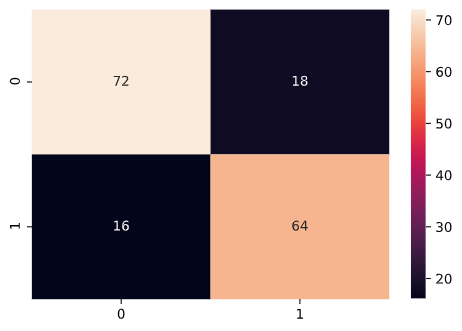
\includegraphics[scale=0.5]{img/matrix-test.png}    
\end{figure}
$$\textbf{SCORE:  } 0.8$$

Como podemos observar, el resultado ha sido lo que esperábamos, y es que ha obtenido prácticamente los mismos valores que los
modelos anteriores. Que haya obtenido un 80\% exacto nos puede hacer pensar que está mal hecho, sin embargo, al tener tan pocos
datos, es posible que se haya dado esto (es más, si miramos la matriz de confusión y sumamos los verdaderos positivos y
negativos, podremos comprobar que es el 80\% exacto del total de ejemplos).

Todas estas ejecuciones y, viendo los resultados que hemos obtenido, lo que nos lleva a pensar es que el modelo está 'atascado'
en este punto. Es decir, que en cuanto a entrenamiento no vamos a obtener muchos mejores resultados con los datos que actualmente
(obviando que podemos crear un modelo que esté sobreajustado de más, algo que tampoco nos conviene). Un conjunto con 961 datos,
de los cuales unos 120 aproximadamente contienen atributos nulos o faltantes, y que a su vez tenemos que dividirlo en datos
para entrenamiento y test; pues es un dataset que se nos queda bastante corto.

Pese a todo esto, con los modelos analizados obtenemos unos porcentajes sobre 80\% de acierto, que es un porcentaje muy bueno.
Con esto quiero decir que, con un dataset más grande y con una o dos características más que sean relevantes para decir si el
tumor es maligno o benigno (aunque esto son temas que no puedo solucionar, ni sé si se puede hacer algo más) pienso que
podríamos obtener unos resultados muy buenos y una tasa de acierto realmente alta.


\newpage

% Pagina de bibliografia
\begin{thebibliography}{}
    
    \bibitem{svc}
    Scikit-Learn. \textit{SVC}
    \\\url{https://scikit-learn.org/stable/modules/generated/sklearn.svm.SVC.html#sklearn.svm.SVC}
    
    \bibitem{random_forest}
    Scikit-Learn. \textit{RandomForestClassifier}
    \\\url{https://scikit-learn.org/stable/modules/generated/sklearn.ensemble.RandomForestClassifier.html#sklearn.ensemble.RandomForestClassifier}
    
    \bibitem{neural_network}
    Scikit-Learn. \textit{MLPClassifier}
    \\\url{https://scikit-learn.org/stable/modules/generated/sklearn.neural_network.MLPClassifier.html#sklearn.neural_network.MLPClassifier}
    
    \bibitem{scaler}
    Scikit-Learn. \textit{StandardScaler}
    \\\url{https://scikit-learn.org/stable/modules/generated/sklearn.preprocessing.StandardScaler.html}
    
    \bibitem{pca}
    Scikit-Learn. \textit{PCA}
    \\\url{https://scikit-learn.org/stable/modules/generated/sklearn.decomposition.PCA.html}
    
    \bibitem{bib:learning_curve}
    Scikit-Learn. \textit{plot\_learning\_curve}
    \\\url{https://scikit-learn.org/stable/auto_examples/model_selection/plot_learning_curve.html#sphx-glr-auto-examples-model-selection-plot-learning-curve-py}
    
    \bibitem{bib:recall}
    Scikit-Learn. \textit{recall\_score}
    \\\url{https://scikit-learn.org/stable/modules/generated/sklearn.metrics.recall_score.html}
    
    \bibitem{bib:precision}
    Scikit-Learn. \textit{precision\_score}
    \\\url{https://scikit-learn.org/stable/modules/generated/sklearn.metrics.precision_score.html}
    
    \bibitem{bib:normalize}
    \textit{Should I normalize/standardize/rescale the data?}
    \\\url{http://www.faqs.org/faqs/ai-faq/neural-nets/part2/}
    
    \bibitem{bib:sensitivity-specifity}
    Wikipedia. \textit{Sensitivity and specifity}
    \\\url{https://en.wikipedia.org/wiki/Sensitivity_and_specificity}
    
    \bibitem{bib:svm-kernels}
    DataFlair. \textit{Kernel Functions-Introduction to SVM Kernel \& Examples}
    \\\url{https://data-flair.training/blogs/svm-kernel-functions/}
    
    \bibitem{bib:loss-nn}
    Isaac Changhau. \textit{Loss Functions in Neural Networks}
    \\\url{https://isaacchanghau.github.io/post/loss_functions/}
    
    \bibitem{bib:svm}
    MathWorks\textit{Support Vector Machine}
    \\\url{https://es.mathworks.com/discovery/support-vector-machine.html}
    
    \bibitem{bib:cross_val_score}
    Scikit-Learn. \textit{cross\_val\_score}
    \\\url{https://scikit-learn.org/stable/modules/generated/sklearn.model_selection.cross_val_score.html}
    
    \bibitem{bib:train_test_split}
    Scikit-Learn. \textit{train\_test\_split}
    \\\url{https://scikit-learn.org/stable/modules/generated/sklearn.model_selection.train_test_split.html}
    
    \bibitem{bib:confusion-matrix}
    Scikit-Learn. \textit{Confusion Matrix}
    \\\url{https://scikit-learn.org/stable/auto_examples/model_selection/plot_confusion_matrix.html}
    
    \end{thebibliography}



\end{document}